\section{Wave Equation}
\label{sec:wave}

We proceed to integrate the HEL Vlasov solver with the wave equation, enabling us to self-consistently investigate resonant wave-particle interactions. In this paper, we focus on the interaction between energetic electrons and chorus waves within the Earth's magnetosphere. Chorus waves are circularly polarized electromagnetic waves that propagate along the Earth's dipole magnetic field. The vector potential A(s, t) representing the transverse wave is expressed as follows:
\begin{equation}
    \mathbf{A}(s,t) = \mathbf{a}(s,t)e^{\imath \phi_f},.
\end{equation}
where $\phi_f$ is the fast varying phase and $\mathbf{a}(s,t)$ is the slowly varying envelope of the wave packet. 
The second order wave equation for the chorus in the resonant frame  is 
\begin{equation}\label{eq.Wave}
    \begin{aligned}
        &\frac{\partial^2 a}{\partial t^2} - \frac{\partial^2 a}{\partial s_i^2} + {2\imath\omega_l}\frac{\partial a}{\partial t} + 2\imath k_l\frac{\partial a}{\partial s_i} + \\
        &\frac{\omega_p^2 \omega_{ce}}{(\omega_{ce}-\omega_l)} \int_0^t d \tau \frac{\partial a}{\partial \tau} e^{-\imath\left(\omega_l-\omega_{c e}\right)(t-\tau)} = {4\pi}j_p~,
        \end{aligned}
      \end{equation}
where $a = a_x + \imath a_y$ with $x$ and $y$ the directions perpendicular to the  magnetic field. 
The plasma current is a combination of contributions from both cold electrons and energetic electrons. The cold electron current can be analytically integrated. We represent the second-order wave equation (\ref{eq.Wave}) as a system of first-order ordinary differential equations, as shown below:
\begin{equation}\label{eq.Wave2}
    \begin{aligned}
        \frac{d y_0}{d t} & = y_1 + D \frac{\partial^2 y_0}{\partial s^2}
        \\
        \frac{d y_1}{d t} & =-2 \imath \omega_l y_1+\frac{\partial^2 y_0}{\partial s^2}-2 \imath k_l \frac{\partial y_0}{\partial s}- \frac{\omega^2_p\omega_{ce}}{\omega_{ce}-\omega_l}y_{2} +j_p\\
        \frac{d y_2}{d t} & =y_1-\imath\left(\omega_l-\omega_{ce}\right) y_2~,
        \end{aligned}
\end{equation}
where we have added a numerical diffusive term with $D$ the diffusive coefficient. The terms $y_0,y_1$ and $y_2$ are
\begin{equation}
    \begin{aligned}
        y_0 &= a(s_i,t)~,
        \\
        y_1 &= \frac{\partial a(s_i,t)}{\partial t}~,
        \\
        y_2 &= e^{-\imath(\omega_l-\omega_{ce})t} \int_0^t\mathrm{d}\tau \frac{\partial a}{\partial \tau} e^{\imath(\omega_l-\omega_{ce})\tau}~.
    \end{aligned}
\end{equation}

For the nonuniform, to ensure the order of precision, a linear combination of finite difference scheme is employed, and the first and second order spatial derivatives are given by 
\begin{equation}
    \frac{\partial f}{\partial z} \approx \frac{f(z_k) - f(z_{k-1})}{z_k-z_{k-1}} + \frac{f(z_k) - f(z_{k+1})}{z_k - z_{k+1}} - \frac{f(z_{k+1}) - f(z_{k-1})}{z_{k+1} - z_{k-1}}~,
\end{equation}
and
\begin{equation}
    \frac{\partial^2 f}{\partial z^2} \approx 2 \left(\frac{f(z_{k-1})}{(z_{k-1}-z_{k})(z_{k-1}-z_{k+1})}+\frac{f(z_{k})}{(z_k-z_{k+1})(z_k-z_{k-1})}+\frac{f(z_{k+1})}{(z_{k+1}-z_{k})(z_{k+1}-z_{k-1})}\right)~.
\end{equation}
The energetic electron current $j_p$ is obtained from the perpendicular velocity moment of energetic particle distribution,
\begin{equation}
    j_p(s_i,t) = - \frac{n_{h0}k_l(t)}{4\pi}\iiint \sqrt{2m_e\omega_{ce}(s)(\mathcal{J}+\Omega+\Pi_i)}f e^{\imath \xi} \rm d \xi \rm d \Omega \rm d \mathcal{J}~,
\end{equation}
where $n_{h0}$ is the density ratio of the energetic electrons to the background cold plasmas.
The coupled ordinary differential equations (\ref{eq.Wave2}) in terms of time are subsequently resolved using the RK method.

To check the contribution of the second order derivatives of slowly varying kernel $a(s_i,t)$ in the wave equation (\ref{eq.Wave}), we further simplify the integral term and obtain the first-order advective wave equation 
\begin{equation}\label{eq.Wave1st}
    \frac{\partial a}{\partial t} + v^l_{g} \frac{\partial a}{\partial s_i} = \frac{2\pi v^l_g}{k_l} j_{p}~,
\end{equation}
where $v_g^l$ is the linear group velocity.
\begin{equation}
    %a^{n+1}_k = a^{n}_k \pm {u_k} (a_{k\pm1}^{n+1} - a_{k}^{n+1})\frac{\Delta t}{\Delta s}
    \begin{aligned}
    a^{n+1}_k &= \left[ S_k^n \pm  \frac{\mathrm{imp}}{\Delta s}  {u_k} a_{k\pm1}^{n+1} + \left(\frac{1}{\Delta t} - \frac{(1- \mathrm{imp})}{\Delta s} u_k\right)  a_{k}^{n} \pm  \frac{(1-\mathrm{imp})}{\Delta s} u_k a_{k \pm 1}^{n} \right]/\left(\frac{1}{\Delta s} + \frac{\mathrm{imp}}{\Delta s}u_k\right)
    \end{aligned}
\end{equation}
where $u_k = v_g(s=s_k)$, $S_k$ is the source term in the right-hand-side of Eq. (\ref{eq.Wave1st}), $\mathrm{imp}$ is the combination factor of the implicit-explicit upwind scheme. 
The sign of the advective term depends on the direction of the group velocity. We apply absorption boundary conditions at one end of the domain and a fixed noisy initialization condition at the other end.

Fig. \ref{fig.cmp2} demonstrates that the first-order wave equation provides a strong approximation to the second-order wave equation. Consequently, the second-order term in Eq. (\ref{eq.Wave}) may be disregarded when simulating the onset of chorus wave frequency chirping for the sake of computational efficiency.
\begin{figure}[htbp]
    \centering
    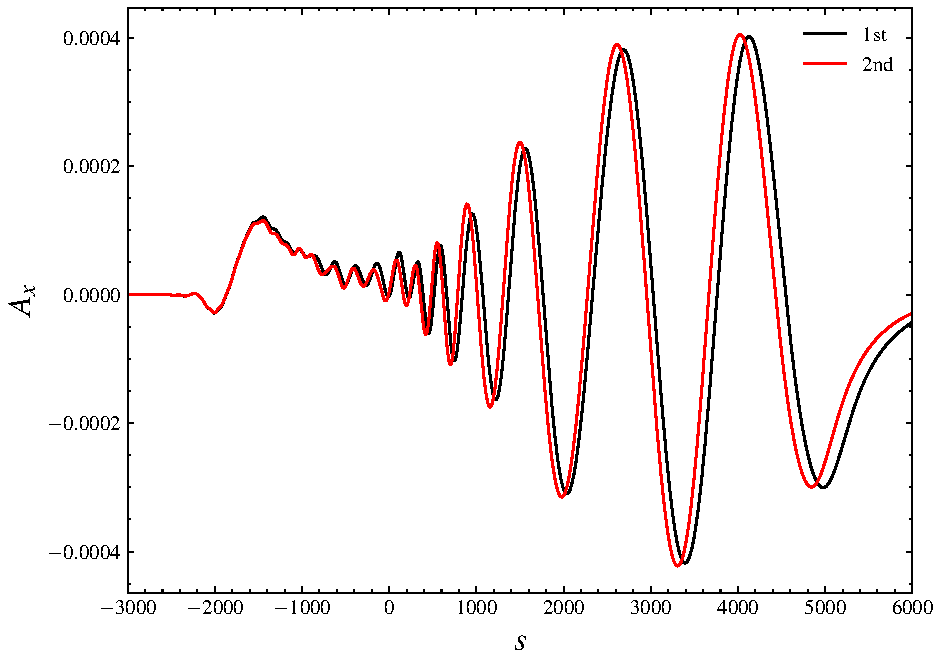
\includegraphics[scale=0.5]{cpc_img/fig_diff.pdf}
    \caption{ Wave amplitudes calculated from the second-order and first-order wave equations. 
    }
    \label{fig.cmp2}
\end{figure}